% Titeseite

\begin{titlepage}
  \begin{center}
	  
    %\mbox{}

    %\vspace{1cm}

	\centering
	
\includegraphics[width=3cm]{figures/tub.pdf}\\
	\vspace{0.8em}
	\LARGE 

	\textsc{Technische Universit\"at Berlin}

    \vspace{1cm}

    \sffamily \LARGE \textbf{Analysis and Optimization of Resource Allocation Mechanism in WiFi Network}

    \vspace{1cm}

    \sffamily \Large \textbf{A quantitative analysis framework for WiFi rate control measurement data}

    \vspace{1.5cm}


    \large \textbf{Submitted by:}
    % \normalsize Submitted by

    \vspace{.1cm}

    \large Elham Aref

    \vspace{.8cm}

  %  von der Fakult�t IV - Elektrotechnik und Informatik der Technischen Universit�t Berlin


    \normalsize Faculty  IV -- Electrical Engineering and Computer Science\\
    %\vspace{.1cm}
    \normalsize Technical University of Berlin\\
    %\vspace{.1cm}
%    \normalsize zur Erlangung des akademischen Grades\\
    %\vspace{.1cm}
%    \large \textsc{Diplom der Ingenieurwissenschaften (Dipl.-Ing.)}\\
    \vspace{.1cm}
   % \normalsize genemigte Diplomarbeit\\
   \normalsize  Master's Thesis\\

    \vspace{1cm}

    \large \textbf{Examiners:}

    \vspace{.2cm}

		\begin{tabular}{rl}
		&Prof. Dr.-Ing. Slawomir Stanczak
, TU-Berlin\\
		&Prof. Dr. Stefan Schmid
, TU-Berlin\\
		\end{tabular}\\

    \vspace{2cm}
    % \large Defense day : 14.2.2023\\
    \vspace{0.5cm}
    \large Berlin 2023\\

  % 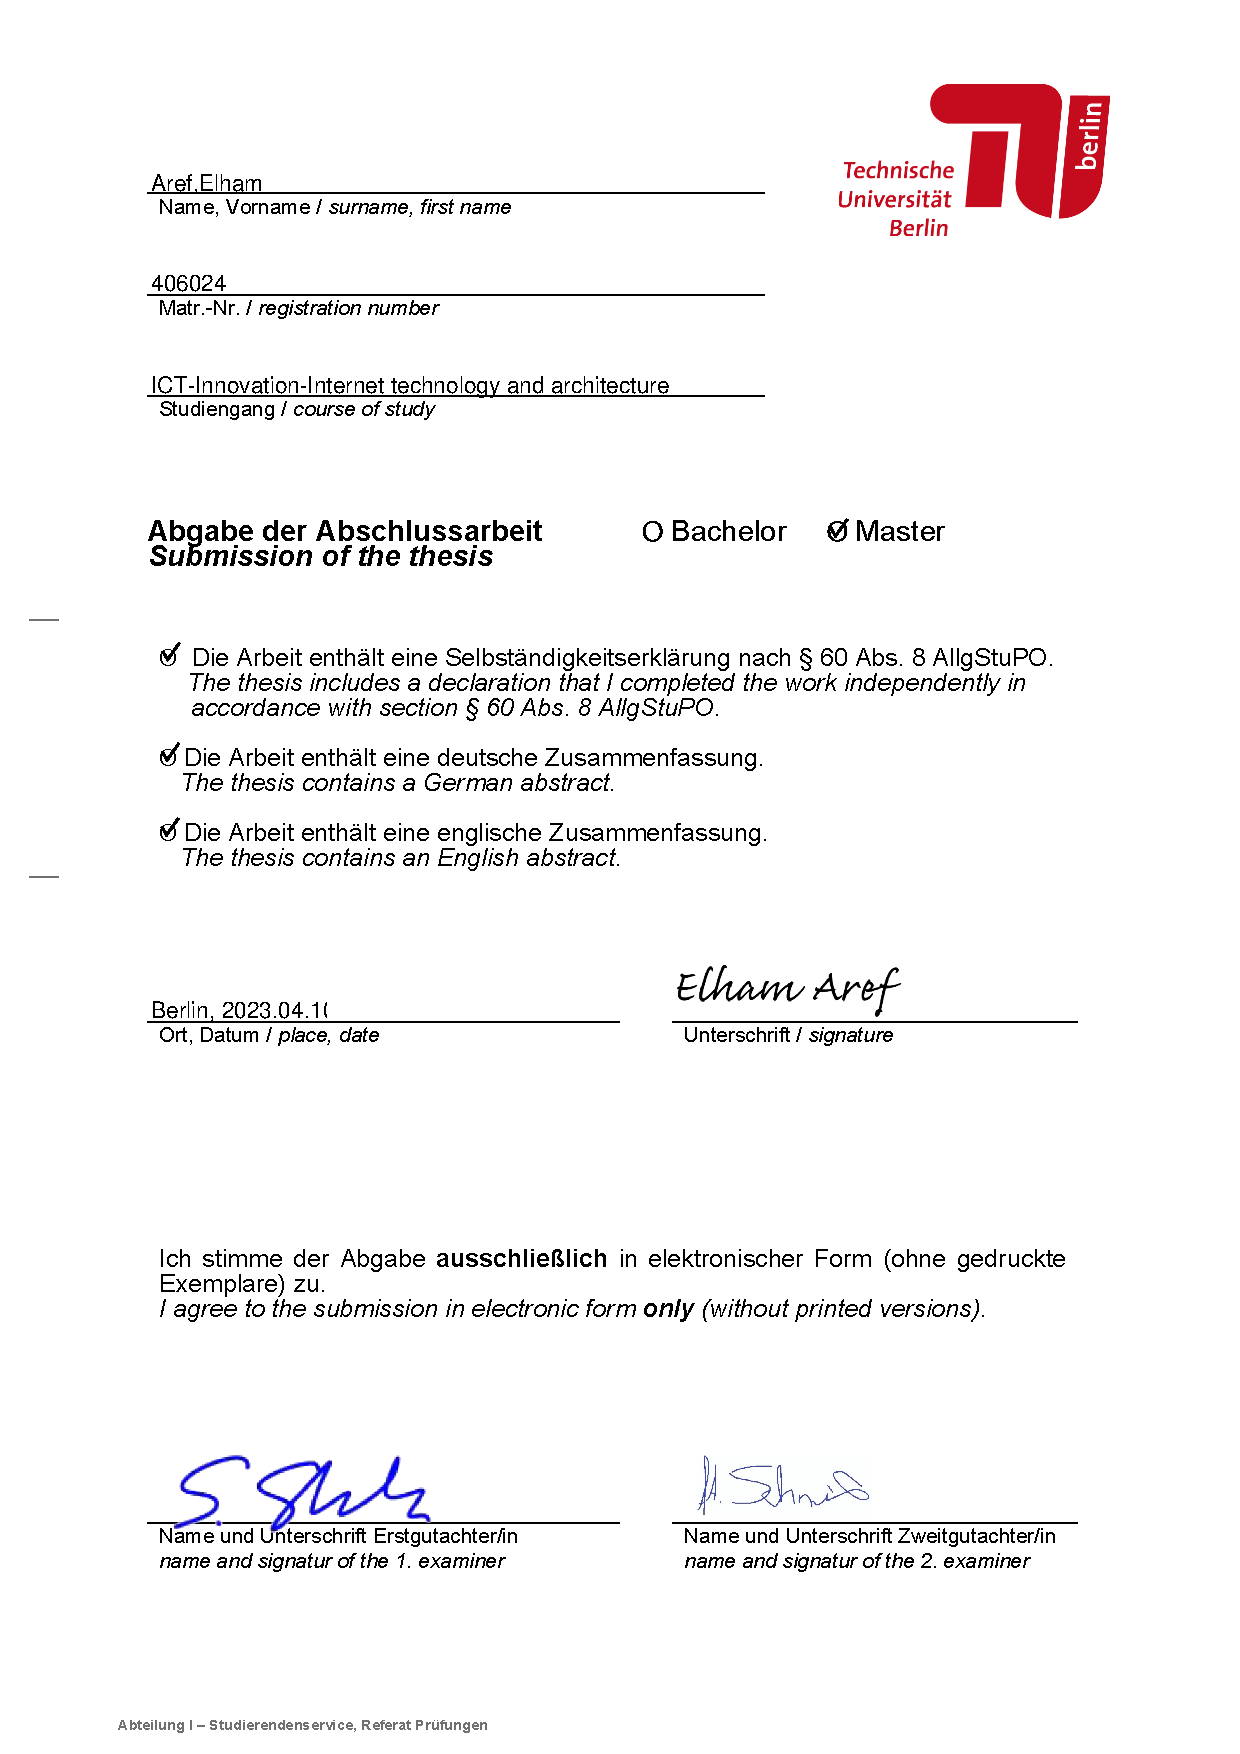
\includegraphics[width=\textwidth]{figures/consent.pdf}

  \end{center}


\end{titlepage}

